\documentclass{article}
\usepackage{tikz}
\usepackage[margin=0.5in,landscape]{geometry}
\usepackage{graphicx}
\usetikzlibrary{arrows.meta,positioning,fit}
\pagestyle{empty}

\begin{document}
\centering
\resizebox{\textwidth}{!}{%
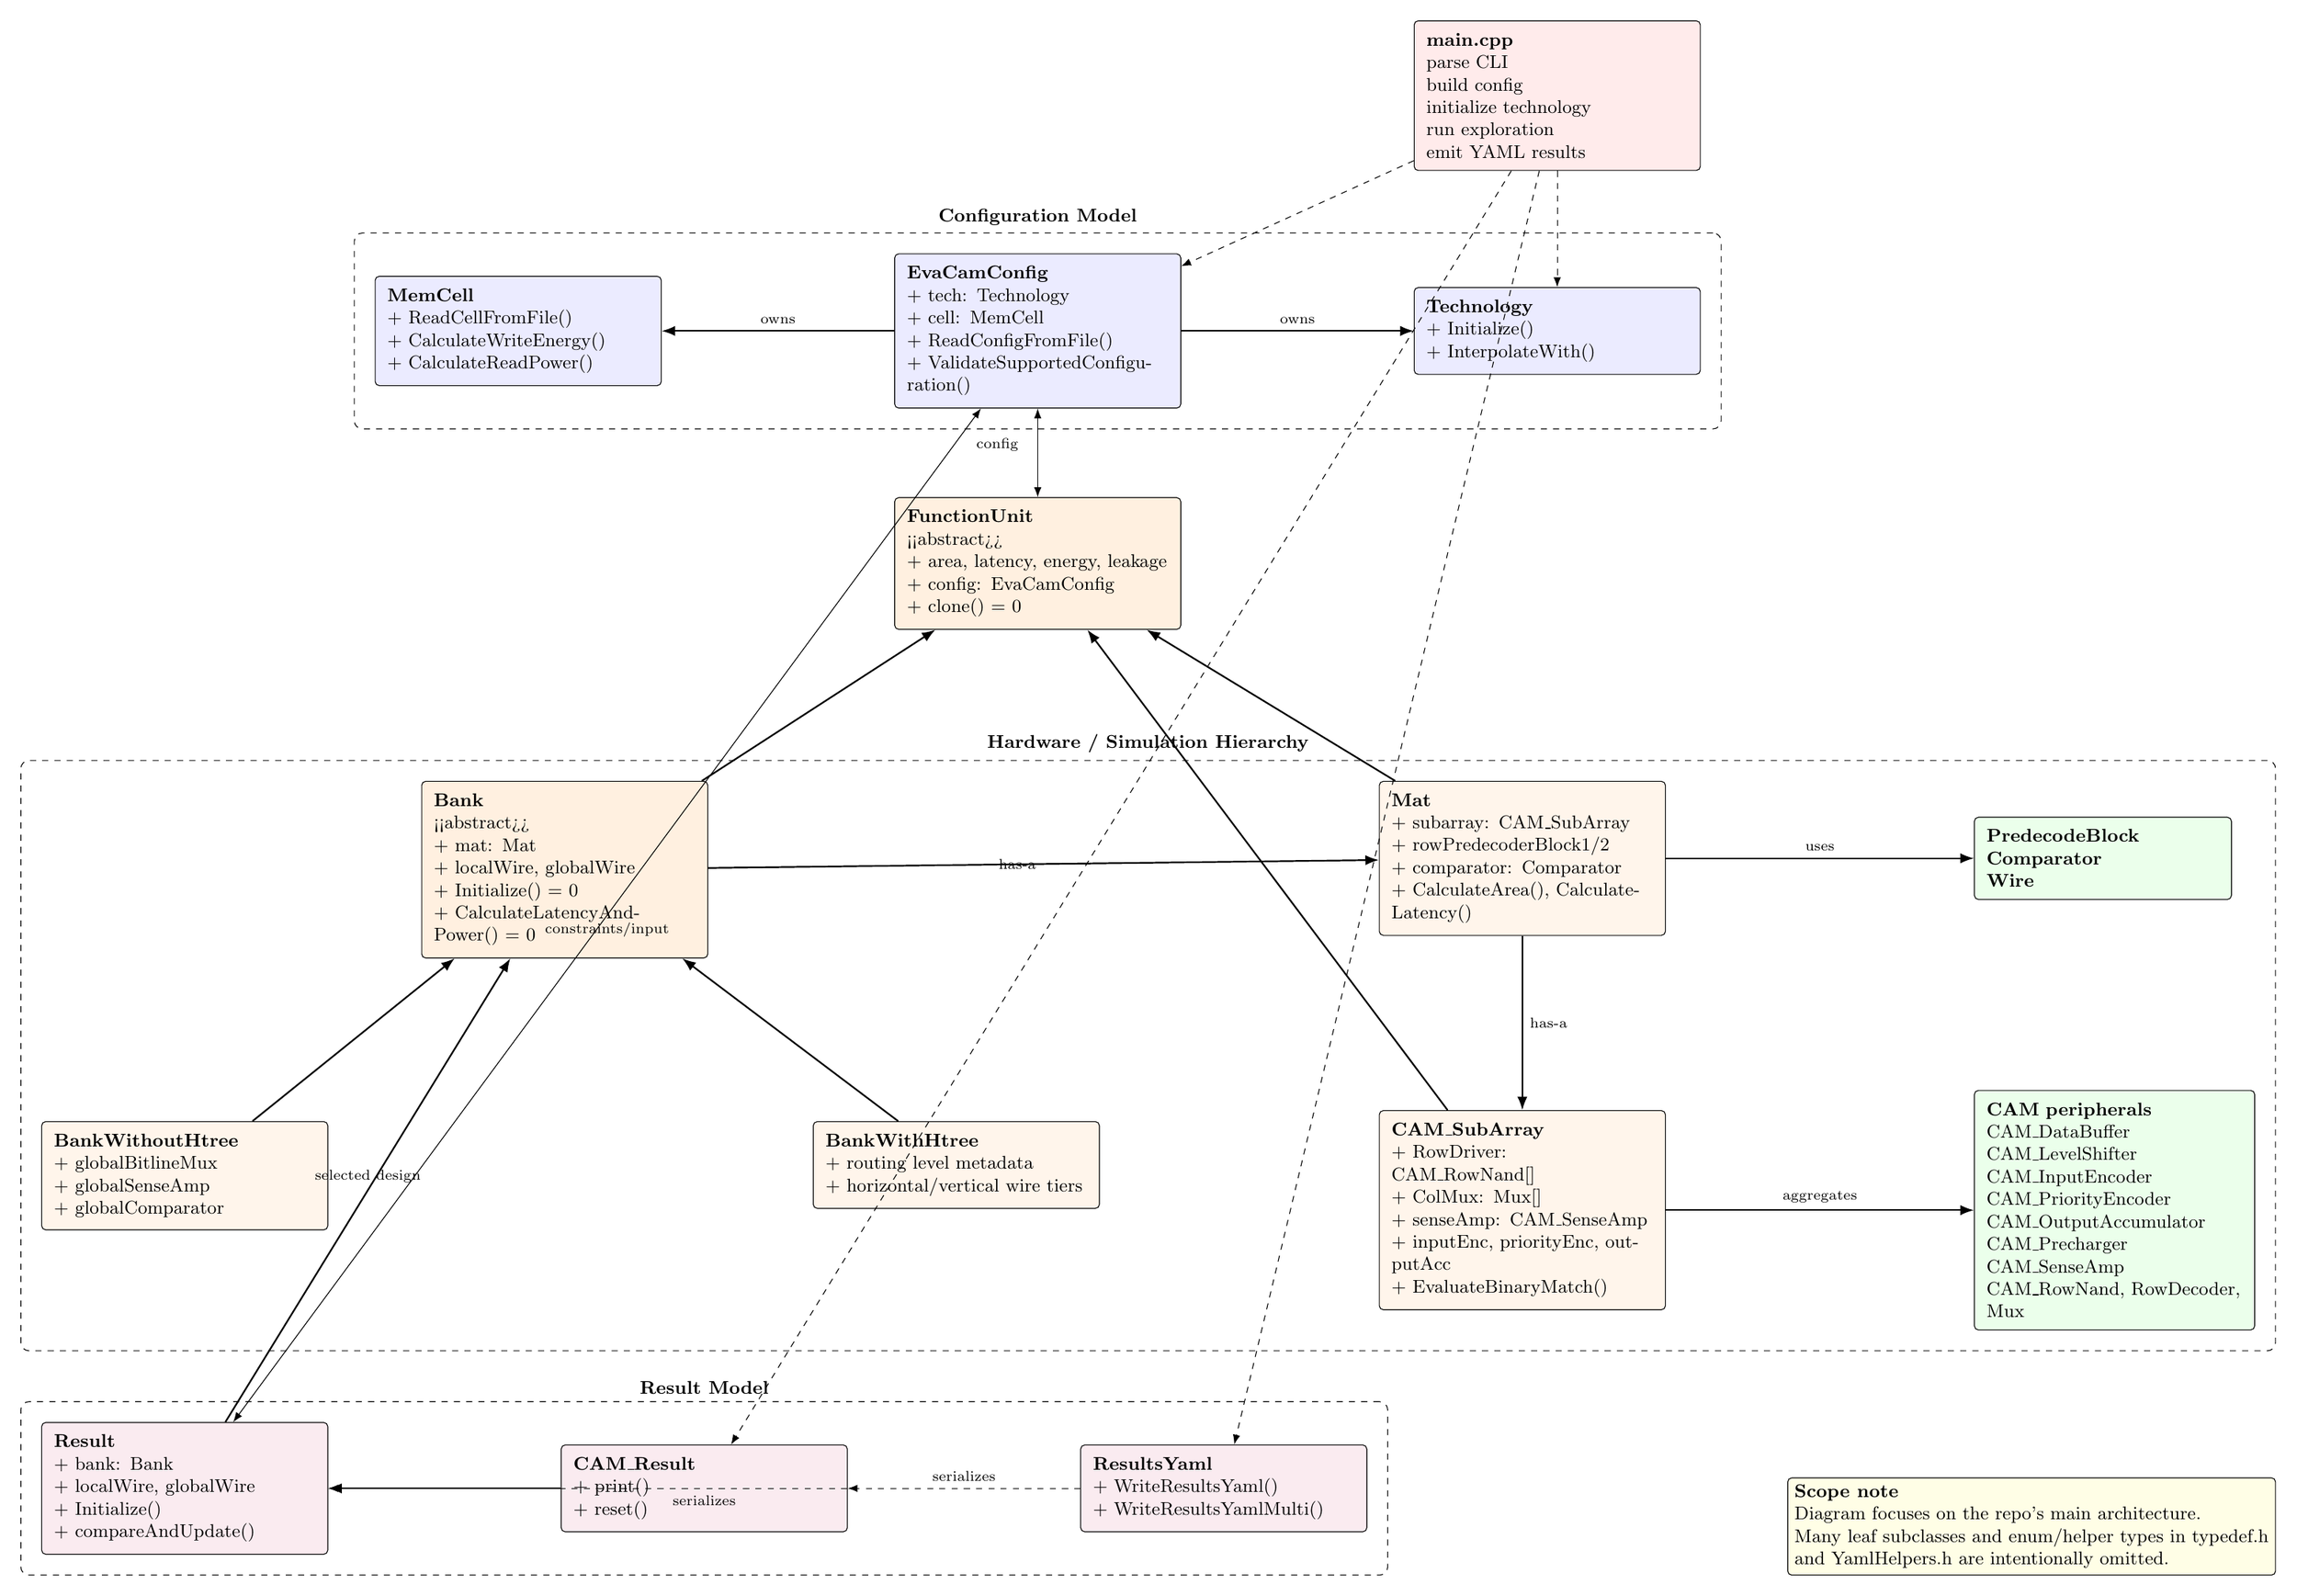
\begin{tikzpicture}[
  font=\small,
  >=Latex,
  class/.style={
    draw,
    rounded corners=2pt,
    align=left,
    minimum width=4.8cm,
    minimum height=1.1cm,
    text width=4.5cm,
    inner sep=6pt,
    fill=white
  },
  abstract/.style={
    class,
    fill=gray!10
  },
  package/.style={
    draw,
    dashed,
    rounded corners=4pt,
    inner sep=10pt
  },
  inherit/.style={-Latex, thick},
  assoc/.style={Latex-Latex, thin},
  owns/.style={-Latex, thick},
  uses/.style={-Latex, dashed}
]

% Core config objects
\node[class, fill=blue!8] (config) at (0, 7.1) {%
  \textbf{EvaCamConfig}\\
  + tech: Technology\\
  + cell: MemCell\\
  + ReadConfigFromFile()\\
  + ValidateSupportedConfiguration()
};

\node[class, fill=blue!8, right=4.0cm of config] (tech) {%
  \textbf{Technology}\\
  + Initialize()\\
  + InterpolateWith()
};

\node[class, fill=blue!8, left=4.0cm of config] (memcell) {%
  \textbf{MemCell}\\
  + ReadCellFromFile()\\
  + CalculateWriteEnergy()\\
  + CalculateReadPower()
};

% Base hierarchy
\node[abstract, fill=orange!12] (fu) at (0, 3.1) {%
  \textbf{FunctionUnit}\\
  <<abstract>>\\
  + area, latency, energy, leakage\\
  + config: EvaCamConfig\\
  + clone() = 0
};

\node[abstract, fill=orange!12, below left=2.6cm and 3.2cm of fu] (bank) {%
  \textbf{Bank}\\
  <<abstract>>\\
  + mat: Mat\\
  + localWire, globalWire\\
  + Initialize() = 0\\
  + CalculateLatencyAndPower() = 0
};

\node[class, fill=orange!8, below right=2.6cm and 3.4cm of fu] (mat) {%
  \textbf{Mat}\\
  + subarray: CAM\_SubArray\\
  + rowPredecoderBlock1/2\\
  + comparator: Comparator\\
  + CalculateArea(), CalculateLatency()
};

\node[class, fill=orange!8, below=3.0cm of mat] (camsub) {%
  \textbf{CAM\_SubArray}\\
  + RowDriver: CAM\_RowNand[]\\
  + ColMux: Mux[]\\
  + senseAmp: CAM\_SenseAmp\\
  + inputEnc, priorityEnc, outputAcc\\
  + EvaluateBinaryMatch()
};

\node[class, fill=orange!8, below left=2.8cm and 1.6cm of bank] (bankwo) {%
  \textbf{BankWithoutHtree}\\
  + globalBitlineMux\\
  + globalSenseAmp\\
  + globalComparator
};

\node[class, fill=orange!8, below right=2.8cm and 1.8cm of bank] (bankwh) {%
  \textbf{BankWithHtree}\\
  + routing level metadata\\
  + horizontal/vertical wire tiers
};

% Peripheral blocks
\node[class, fill=green!8, right=5.3cm of mat, text width=4.0cm, minimum width=4.3cm] (predecode) {%
  \textbf{PredecodeBlock}\\
  \textbf{Comparator}\\
  \textbf{Wire}
};

\node[class, fill=green!8, right=5.3cm of camsub, text width=4.4cm, minimum width=4.7cm] (periph) {%
  \textbf{CAM peripherals}\\
  CAM\_DataBuffer\\
  CAM\_LevelShifter\\
  CAM\_InputEncoder\\
  CAM\_PriorityEncoder\\
  CAM\_OutputAccumulator\\
  CAM\_Precharger\\
  CAM\_SenseAmp\\
  CAM\_RowNand, RowDecoder, Mux
};

% Result side
\node[class, fill=purple!8, below=3.3cm of bankwo] (result) {%
  \textbf{Result}\\
  + bank: Bank\\
  + localWire, globalWire\\
  + Initialize()\\
  + compareAndUpdate()
};

\node[class, fill=purple!8, right=4.0cm of result] (camresult) {%
  \textbf{CAM\_Result}\\
  + print()\\
  + reset()
};

\node[class, fill=purple!8, right=4.0cm of camresult] (yaml) {%
  \textbf{ResultsYaml}\\
  + WriteResultsYaml()\\
  + WriteResultsYamlMulti()
};

% Entry point
\node[class, fill=red!8, above=2.0cm of tech] (main) {%
  \textbf{main.cpp}\\
  parse CLI\\
  build config\\
  initialize technology\\
  run exploration\\
  emit YAML results
};

% Relationships
\draw[owns] (config) -- node[above] {\scriptsize owns} (tech);
\draw[owns] (config) -- node[above] {\scriptsize owns} (memcell);
\draw[assoc] (fu) -- node[left, xshift=-6pt, yshift=4pt] {\scriptsize config} (config);

\draw[inherit] (bank) -- (fu);
\draw[inherit] (mat) -- (fu);
\draw[inherit] (camsub) -- (fu);
\draw[inherit] (bankwo) -- (bank);
\draw[inherit] (bankwh) -- (bank);

\draw[owns] (bank) -- node[left] {\scriptsize has-a} (mat);
\draw[owns] (mat) -- node[right] {\scriptsize has-a} (camsub);
\draw[owns] (mat) -- node[above] {\scriptsize uses} (predecode);
\draw[owns] (camsub) -- node[above] {\scriptsize aggregates} (periph);

\draw[owns] (result) -- node[above] {\scriptsize selected design} (bank);
\draw[assoc] (result) -- node[below] {\scriptsize constraints/input} (config);
\draw[inherit] (camresult) -- (result);
\draw[uses] (yaml) -- node[above] {\scriptsize serializes} (camresult);
\draw[uses] (yaml) -- node[below] {\scriptsize serializes} (result);

\draw[uses] (main) -- (config);
\draw[uses] (main) -- (tech);
\draw[uses] (main) -- (camresult);
\draw[uses] (main) -- (yaml);

% Package outlines
\node[package, fit=(config)(tech)(memcell), label=above:{\textbf{Configuration Model}}] {};
\node[package, fit=(bank)(mat)(camsub)(bankwo)(bankwh)(predecode)(periph), label=above:{\textbf{Hardware / Simulation Hierarchy}}] {};
\node[package, fit=(result)(camresult)(yaml), label=above:{\textbf{Result Model}}] {};

% Legend / scope note
\node[draw, rounded corners=2pt, fill=yellow!10, align=left, anchor=south east] at (current bounding box.south east) {%
  \textbf{Scope note}\\
  Diagram focuses on the repo's main architecture.\\
  Many leaf subclasses and enum/helper types in typedef.h\\
  and YamlHelpers.h are intentionally omitted.
};

\end{tikzpicture}
}
\end{document}
